%!TEX root = ../Thesis.tex
\section{Planar Intersection Algorithm}

- assume satellite is at infinity for comparing difference in pseudorange for a particular reference satellite.\\
- use all satellites as reference satellite - no single point of failure, also not all satellites might be in view for all receivers\\
- get the normal vector between all receivers and each sat. \\
- Calculate the average normal vector.\\
- get the difference in pseudorange between all receivers along each normal vector \\
- create a plane with the normal vector with that distance\\
- solve via optimization (least squares) \\
- use clock adjustment from abs gps? or have as another optimisation variable\\
- antenna problems? misalignment?\\
- share clock bias's between solving for different reference sets? - do it one by one or all together?\\
- need to align the time of signal sent to the receivers before calculating average normal vector\\

- have weighted planes based on ? have weighted area on the planes?\\
- if one plane intercepts far away from the others then ignore it (multipath). hyperdimensional surface to minimise




% conceptual
how to send data between receivers? do it offline on a different platform?


https://www.e-education.psu.edu/geog862/node/1759 - errors in pseduorange

http://www.insidegnss.com/node/2898 - how to get pseudorange from raw data

\subsection{Assumptions}
\subsubsection{Static Receivers}
All receivers are static for the time in between all receivers get a GPS lock. This makes for an easier transform to align the satellite positions to a common time. It also ignores the problem of how the pseudorange from each receiver would be sent to either all of the receivers or to a central device for computation and the time delay associated with that. The incorporation of moving receivers is an area to explore for future work on the algorithm.

\subsubsection{Transform asynchronous time}
any two receivers will not be synchronized. The earliest time between all the receivers will be used as the time reference point. The satellite position in the future time steps were backcalculated to find the difference in the pseudorange. As the time between receivers will be $\approx$ 1 second, this extra distance is only in the vacuum of space and is not affected by potential nonlinear affects such as ionosphere and troposphere errors that affect the speed of light.\\

The error in the normal vector due to the time difference is

There have been many advances in the field, therefore to test the planar algorithm itself it is assumed that the asynchronous time is transformed to a common epoch time.

\subsubsection{Parallel plane assumption}
It as assumed for the plane equations that all receivers point to a satellite along the same vector. This is valid for a dispersion of receivers for 10km for an error of XX. This is synonymous to if the satellites were at infinity and all the receiver vectors are parallel to a satellite



\begin{eqnarray}
\delta &=& \tan^{-1}\left(\frac{d}{a}\right) \label{Eq:parplane delta}\\
e &=& 2d\tan\delta \label{Eq: parplane e(d)}\\
\eqref{Eq:parplane delta} \& \eqref{Eq: parplane e(d)}\Rightarrow e&=&\frac{2d^2}{a}
\end{eqnarray}
Where a is the altitude, d is the distance between two receivers and e is the error in the plane created. The worst configuration for error in the vector normal to the plane is if the satellite is directly above the receivers at the smallest distance from the Earth in orbit, $a>20000\;km$. For d=5 km the perpendicular error is 2.5 m




\subsection{Algorithm}

\subsubsection{Pre-Processing}
\paragraph{Select reference receiver $\alpha$}
The receiver $\alpha$ is used as the reference location and common time in the NED frame. 
\paragraph{Collect data of one timestep from all receivers}
The raw data as well as the estimated absolute location and clock bias (what frame of reference is this?) from non-linear least squares optimisation is collected from all GNSS receivers.
\paragraph{Align to reference Epoch time}\label{timetransform}


\subsubsection{Distance Optimisation}
By optimising the distance between each pair of receivers, the error in the whole system is minimised. 
This means that the position receivers are not only relative to the reference receiver $\alpha$ but between all receivers just with the reference frame origin located at $\alpha$. It is because of this step a receiver does not need to have all the same satellites in view as all other receivers, including the designated $\alpha$.


\paragraph{Average normal Vector}
Find the average normal vector pointing to each satellite $\hat{\eta_s}$ from the receivers. The normal vector is calculated by using the position all of the satellites in view at the common time $t_{\alpha}$ as previously transformed in \ref{timetransform} and the estimated absolute position of all receivers. The average for each satellite is calculated by taking the mean across all receivers.

\paragraph{Difference in Pseudorange}
The differences in pseudorange are calculated $\Delta\rho^s_{\omega_i\omega_j}$ where s is the satellite, $\omega_i$ and $\omega_j$ are receivers $(for i<j, i\neq j)$. 

\paragraph{Optimise Pseudorange}
The pseudorange between each pair of receivers along each normal vector $\hat{\eta_s}$ creates an overdetermined linear system that is solved via least squares.
\begin{figure}
\centering
\caption{text}
\label{key}
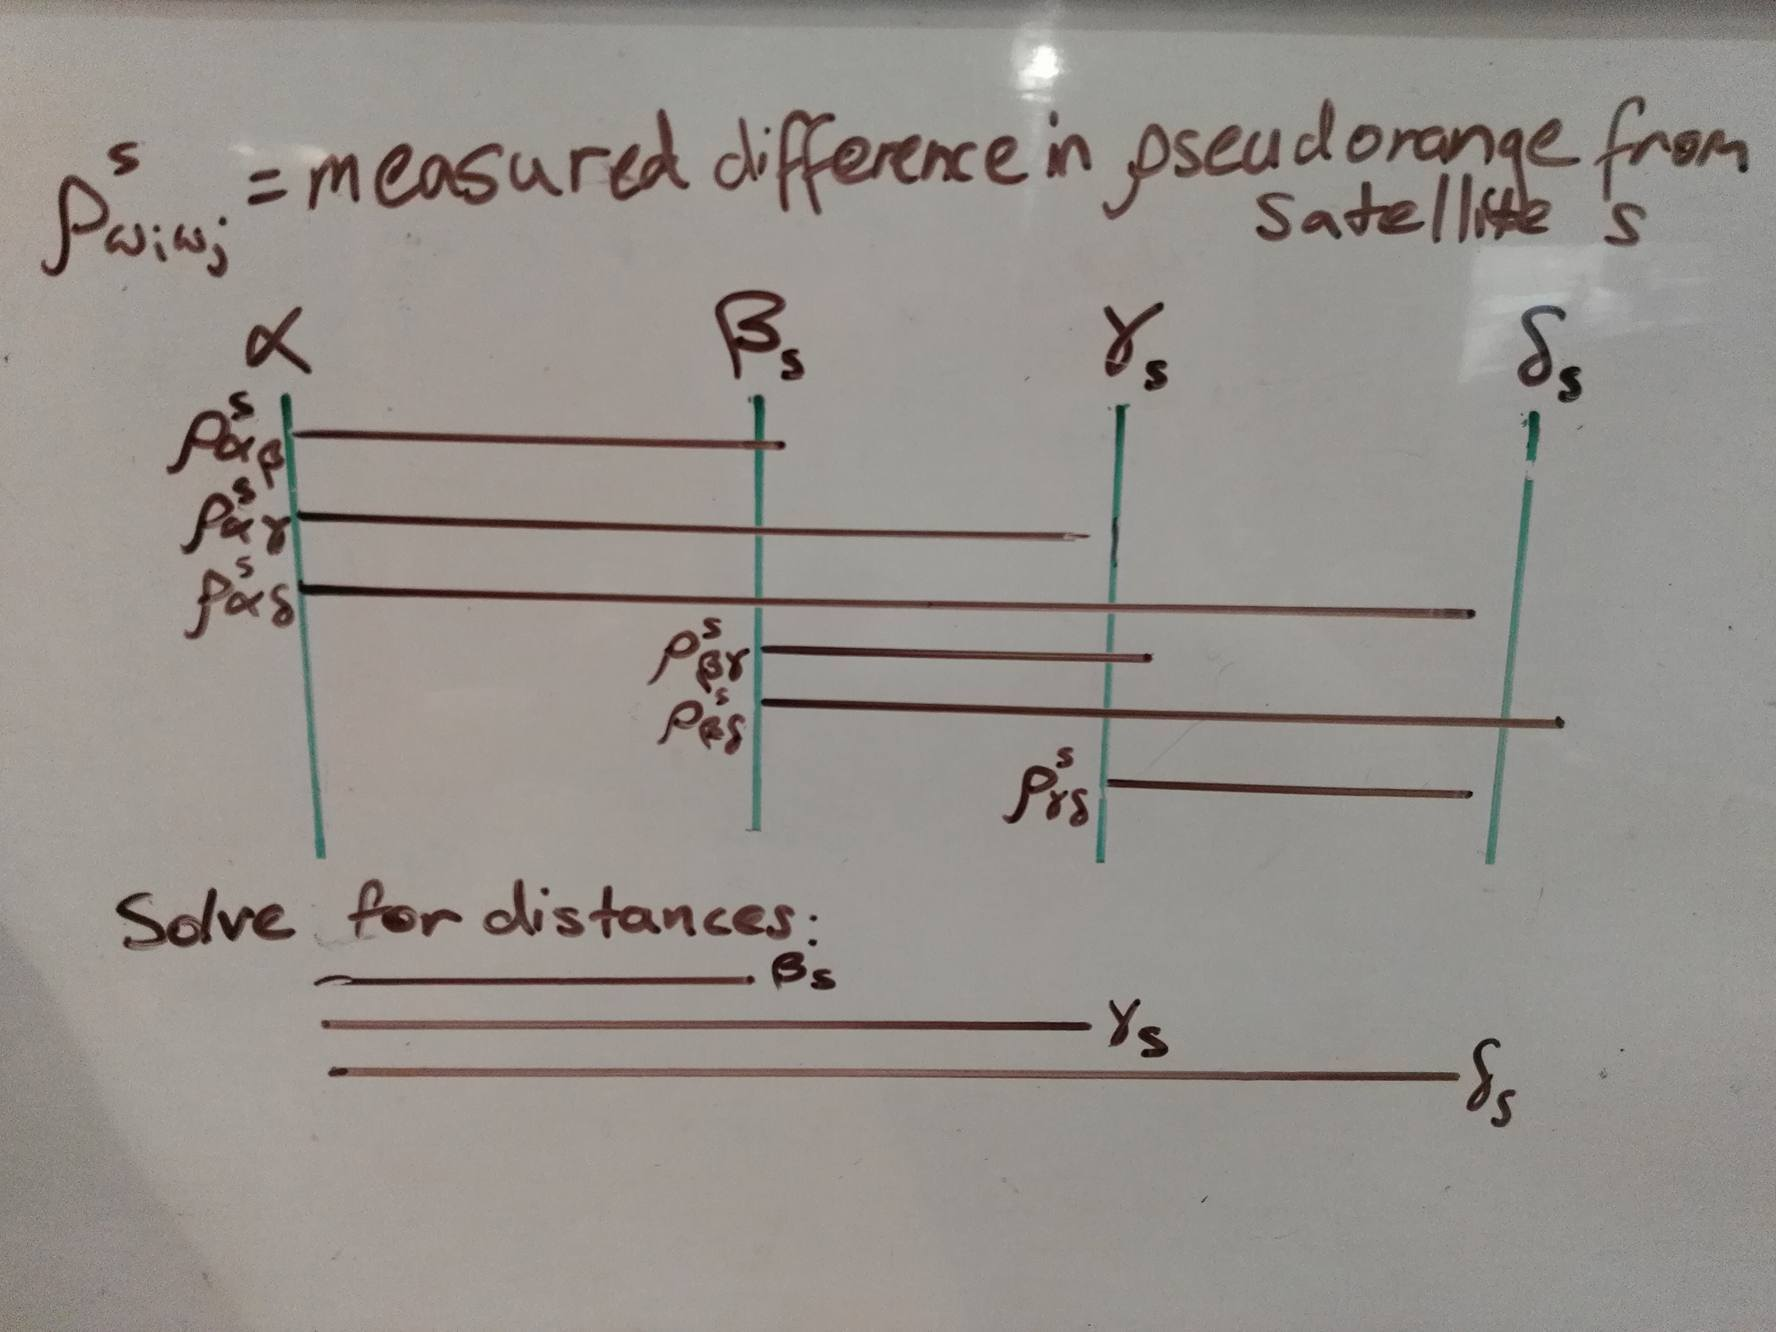
\includegraphics[width=0.7\linewidth]{ChapterPerception/Figures/solve_distances.jpg}
\end{figure}
\begin{eqnarray}
\Phi &=& \begin{bmatrix}
0 & -1 & 0 & ...\\
0 & 0 & -1 & ...\\
... & ... & ... & ... \\
1 & -1 & 0 & ...\\
1 & 0 & -1 & ...\\
\hdotsfor{4} \\
0 & 1 & -1 & ...
\end{bmatrix} \\
%
\Omega_s &=& \begin{bmatrix}
\beta_s \\
\gamma_s\\
\delta_s \\
\vdots
\end{bmatrix} \\
%
\rho_s &=& \begin{bmatrix}
\rho_{\alpha\omega_1}\\
\rho_{\alpha\omega_2}\\
\hdotsfor{1}\\
\rho_{\omega_1\omega_2}\\
\rho_{\omega_1\omega_3}\\
\vdots
\end{bmatrix} 
\end{eqnarray}

\begin{eqnarray}
\Phi\times\Omega_s = \rho_s
\end{eqnarray}
Solve by linear least squares for an overdetermined system by the pseudo inverse matrix
\begin{eqnarray}
\Omega_s = (\Phi^T\Phi)^{-1}\Phi^T\rho_s
\end{eqnarray}

\subsubsection{Point Optimisation}
\paragraph{Create Planes}
Create sets of planes for each receiver $\omega$ from the normal vectors $\hat{\eta_s}$ and the set of distances from the reference point $\alpha$ to receiver $\omega$ along each of the normal vectors denoted $\Omega_\omega$.

The equation of a plane is $Ax+By+Cz+D=0$ where the coefficients [A,B,C] describe the normal vector of the plane and the coefficient D sets the plane in 3D space along the vector. As the normal vector is already calculated for each satellite, only the D coefficient must be solved for each receiver and satellite pair. 
\begin{eqnarray}
P_\omega^s &=& (i\cdot\hat{\eta_s})x + (j\cdot\hat{\eta_s})y + (k\cdot\hat{\eta_s})z + D_\omega^s \label{genplane}\\
P_\omega^s &=& I\cdot H +D_\omega\\
\end{eqnarray}
Where $I = x\hat{\textbf{i}}+y\hat{\textbf{j}}+z\hat{\textbf{k}}$ is the *identity* vector and H is a matrix of normal vectors to each satellite:
\begin{eqnarray}
H = \begin{bmatrix}
\hat{\eta_1} \\
\hat{\eta_2} \\
\vdots\\
\hat{\eta_n}
\end{bmatrix}
\end{eqnarray}
The coefficient D can be calculated by finding a point on the plane $f_\omega^s$, then substituting it into \eqref{genplane} for x,y,z. The point of the plane is calculated by moving along the normal vector by the optimised pseudo distance from the reference point \eqref{Eq:f}.
\begin{eqnarray}
f_\omega^s &=& \Delta_\omega^s\hat{\eta_s} \label{Eq:f}\\
P_\omega^s &=& \hat{\eta_s}\cdot f_\omega^s +D_\omega^s = 0\\
D_\omega^s &=& -\hat{\eta_s}\cdot f_\omega^s\\
D_\omega^s &=& -\Delta_\omega^s ||\hat{\eta_s}|| \\
||\hat{\eta_s}|| &=& 1\\
D_\omega^s &=& -\Delta_\omega^s\\
\Rightarrow P_\omega^s &=& I\cdot H -\Omega_\omega
\end{eqnarray}

\begin{figure}[h]
\centering
\caption{Find position $f_\omega^s$ on the plane}
\label{fig:pointonplane}
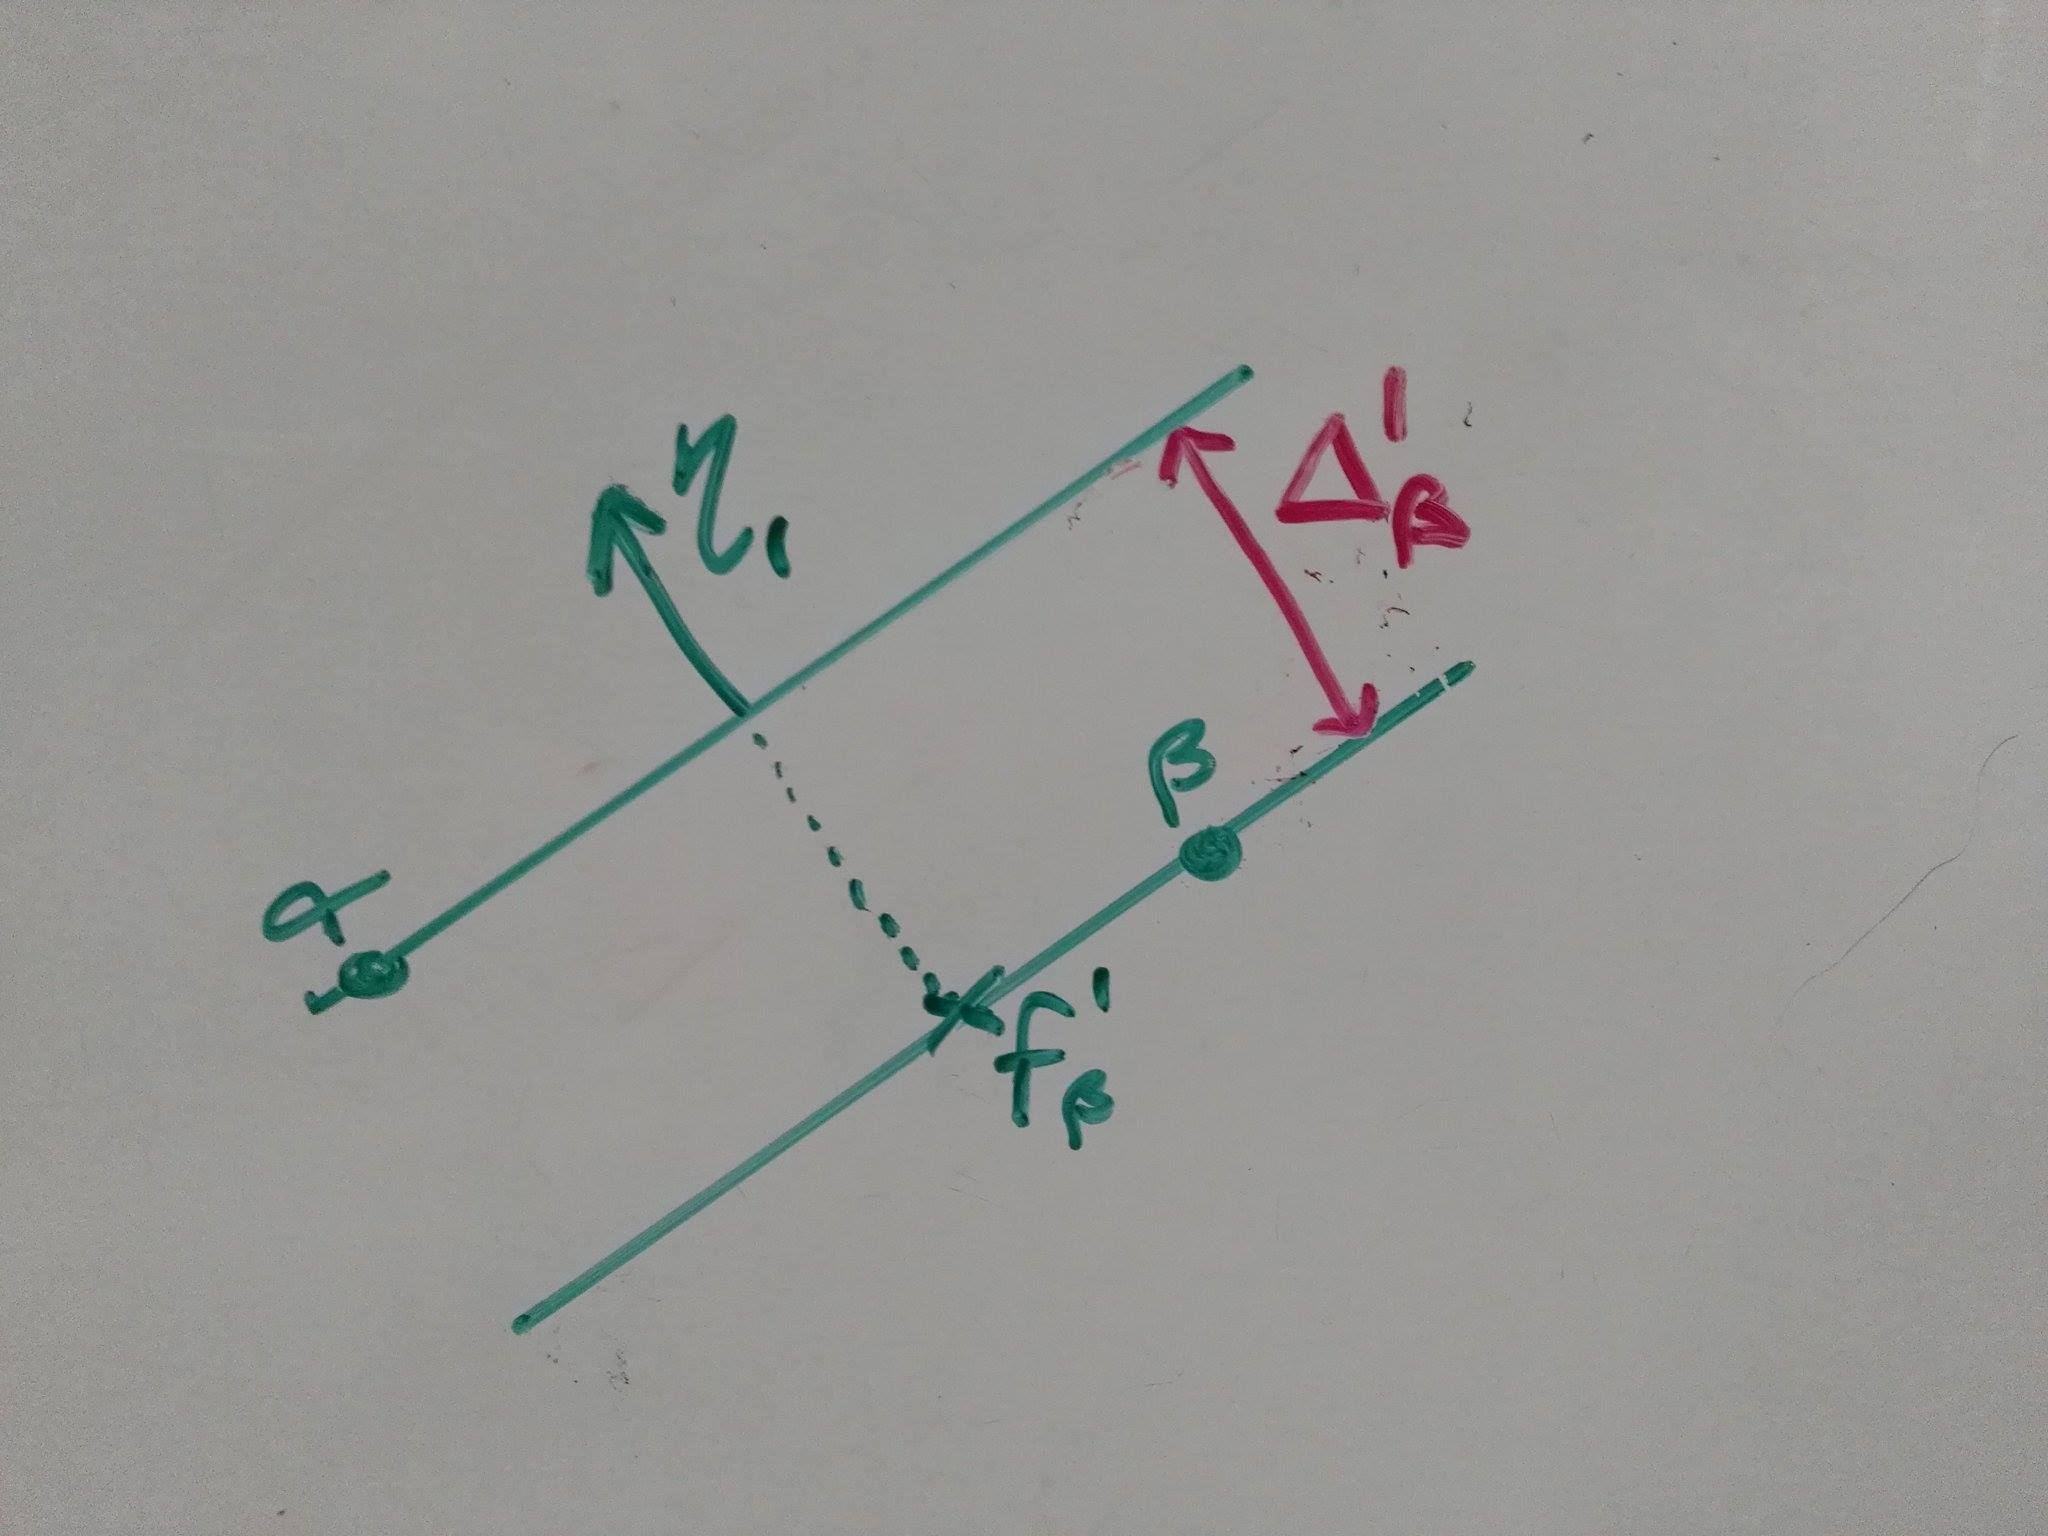
\includegraphics[width=0.7\linewidth]{ChapterPerception/Figures/pointonplane}
\end{figure}






$\Omega_\omega$ is a vector of optimised pseudo-distances from reference $\alpha$ to receiver $\omega$ for all satellites $s\in{1,2...n}$
\begin{eqnarray}
\Omega_\omega = \begin{bmatrix}
\Delta_{\omega}^1 \\
\Delta_{\omega}^2 \\
\vdots\\
\Delta_{\omega}^n \\
\end{bmatrix}
\end{eqnarray}
Where $\Omega_s$ is the vector of optimised pseudo-distances from $\alpha$ to each receiver $\omega\in1,2...m$ for a single satellite s:
\begin{eqnarray}
\Omega_s = \begin{bmatrix}
\Delta_{\omega_1}^s \\
\Delta_{\omega_2}^s \\
\vdots\\
\Delta_{\omega_m}^s \\
\end{bmatrix}
\end{eqnarray}


\paragraph{Solve for Intersection}
As the system of homogeneous linear equations is overdetermined, it can be solved using singular value decomposition to find a point that has the minimum residuals from all of the planes in its set $P_\omega$. Each set of planes for a particular receiver is independent to all other receivers. The vector $X_\omega$ describes the position of receiver $\omega$ in NED coordinates and $\tau_\omega$ describes a final receiver clock bias that alters the displacement of all the planes in the set $P_\omega$ by the same parameter.
\begin{eqnarray}
X_\omega &=& \begin{bmatrix}
x_\omega \\y_\omega \\ z_\omega \\ \tau_\omega
\end{bmatrix}\\
P_\omega X_\omega &=& D_\omega \\
\end{eqnarray}
In order to solve all of the receivers with the least amount of error in the whole system, all of the position vectors $X_\omega$ are solved at the same time. The reference planes of $\alpha$ must be included as a constraint on the system. All of the clock biases are also constrained with the clock bias from $\tau_\alpha$, see \eqref{Eq: P with alphat}.
The receiver clock bias only affects the equation of the planes by altering the constant as a change in the pseudorange has no affect over the angle of the plane. Each receiver clock bias alters all the planes associated with that receiver proportionally. 
\begin{eqnarray}
P_\omega^s &=& (i\cdot\hat{\eta_s})x + (j\cdot\hat{\eta_s})y + (k\cdot\hat{\eta_s})z + D_\omega^s + (\tau_\omega-\tau_\alpha) \label{Eq: P with alphat}\\
\end{eqnarray}
 

